\documentclass[aspectratio=169]{beamer}

%-------------------------------------------------------------
% BASE PACKAGES AND THEMES
%-------------------------------------------------------------
\usetheme{Madrid}
\usecolortheme{default}
\usepackage{hyperref}
\usepackage{tikz}
\usepackage{pgfplots}
\pgfplotsset{compat=1.17}
\usepackage{amsmath, amssymb}
\usepackage{graphicx}

%-------------------------------------------------------------
% BIBLIOGRAPHY CONFIGURATION (fixed)
%-------------------------------------------------------------
\usepackage[
  backend=biber,
  style=ieee,
  citestyle=numeric,
  sorting=none
]{biblatex}

\addbibresource{bib.bib}

%-------------------------------------------------------------
% UNIVERSAL AUTO-FIT SETTINGS FOR PLOTS
%-------------------------------------------------------------
\pgfplotsset{
  every axis/.append style={
    scale only axis,
    width=\dimexpr\linewidth-1em,
    height=0.45\textheight,
    enlarge x limits=0.05,
    enlarge y limits=0.05,
    tick label style={font=\footnotesize},
    label style={font=\footnotesize},
    title style={font=\footnotesize},
  },
}

%-------------------------------------------------------------
% TITLE PAGE INFORMATION
%-------------------------------------------------------------
\title{CMSC 190 Part 1}
\subtitle{Forecasting Weekly Dengue Cases by Integratin Google Earth Engined Based Risk Prediction and Cloud Based Learning}
\author{Nathaniel Aquino}
\institute{University of the Philippines - Baguio}
\date{\today}

%-------------------------------------------------------------
\begin{document}

\begin{frame}
  \titlepage
\end{frame}

\begin{frame}{Overview}
  \tableofcontents
\end{frame}

%------------------------------------------------
\section{Review Related Literature}
%------------------------------------------------

%------------------------------------------------
\subsection{Neural Networks}
%------------------------------------------------
\begin{frame}{Related Literature Review: Neural Networks}

  \begin{itemize}
    \item \textbf{Neural Network:}
      \begin{quote}
        "A neural network is a massively parallel distributed processor made up of simple processing units, which has a natural propensity for storing experiential knowledge and making it available for use." \cite{haykin1999}
      \end{quote}
    \item \textbf{Neuron (Biological):}
      \begin{quote}
        "The neuron is the basic signaling unit of the nervous system... Neurons are specialized for sending signals over long distances... They communicate with one another at specialized contact points called synapses." \cite{kandel2000}
      \end{quote}
    \item \textbf{Network (General Definition):}
      \begin{quote}
        "A network is a collection of objects (nodes) connected by links (edges)." \cite{barabasi2016}
      \end{quote}
  \end{itemize}
\end{frame}

\begin{frame}{Related Literature Review: Neural Network}
  \begin{figure}
    \centering
    \includegraphics[width=0.8\textwidth, keepaspectratio]{assets/biologicalnn.png}
  \end{figure}
\end{frame}

\begin{frame}{Review Literature Review: Artificial Neural Network}
  \framesubtitle{Definitions}

  \begin{block}{Zhang et al. (2016)}
    An artificial neural network (ANN) mimics the human brain in processing input signals and transforms them into output signals. It is a modelling algorithm that allows for non-linearity between feature variables and output signals.
  \end{block}

  \begin{block}{Maind \& Wankar (2014)}
    An artificial neural network is an information-processing paradigm inspired by the way biological nervous systems process information. It consists of a large number of highly interconnected processing elements (neurons) working in unison to solve specific problems.
  \end{block}

\end{frame}

\begin{frame}{Key Components of a Neuron}
  \framesubtitle{Core definitions and their roles}

  \begin{itemize}
    \item \textbf{Inputs ($x$)}
      \begin{itemize}
        \item A vector of numeric feature values (e.g., pixel data, predictors) fed into a neuron at a given time step \cite{goodfellow2016}.
      \end{itemize}
      \vspace{1em}

    \item \textbf{Weights ($w$)}
      \begin{itemize}
        \item Adjustable parameters that scale the influence of each input. They determine the strength and direction of the connection between neurons \cite{goodfellow2016, haykin1999}.
      \end{itemize}
      \vspace{1em}

    \item \textbf{Bias ($b$)}
      \begin{itemize}
        \item An additive parameter that shifts the activation function, allowing the neuron to activate even if all inputs are zero. It is added to the weighted sum of inputs \cite{goodfellow2016}.
      \end{itemize}
      \vspace{1em}

    \item \textbf{Activation Function ($\phi$)}
      \begin{itemize}
        \item A non-linear function (like Sigmoid, Tanh, or ReLU) applied to the neuron's weighted sum plus bias ($a = \phi(z)$) to introduce non-linearity, which allows the network to learn complex patterns \cite{goodfellow2016, nair2010rectified}.
      \end{itemize}
  \end{itemize}

\end{frame}

\begin{frame}{Related Literature Review: Neural Network}
  \begin{figure}
    \centering
    \includegraphics[width=0.5\textwidth, keepaspectratio]{assets/simpleANN.png}
  \end{figure}
\end{frame}

%------------------------------------------------
\subsection{Forward Propagation}
%------------------------------------------------
\begin{frame}{Related Literature Review: Forward Propagation}

  \begin{columns}[c] % 'c' centers content vertically

    \column{.5\textwidth} % Left column for text

    \textbf{Schmidhuber (2015):}

    \vspace{1em} % Adds a bit of space

    \textit{Characterizes forward propagation in deep networks as computing each neuron’s output by applying an activation to an affine transformation of its inputs, layer by layer from inputs to outputs.}

    \column{.5\textwidth} % Right column for image
    \begin{figure}
      \centering
      % \linewidth scales the image to the width of this column
      \includegraphics[width=\linewidth, keepaspectratio]{assets/ANN.png}
    \end{figure}

  \end{columns}

\end{frame}

\begin{frame}{Related Literature Review: Forward Propagation}
  \begin{block}{Schmidhuber (2015)}
    characterizes forward propagation in deep networks as computing each neuron’s output by applying an activation to an affine transformation of its inputs, layer by layer from inputs to outputs.
  \end{block}
\end{frame}

\begin{frame}{Related Literature Review: Forward Propagation and Activation}
  \framesubtitle{The flow of prediction and introducing non-linearity}
  \begin{columns}[c]
    \column{.5\textwidth}
    \textbf{Forward Pass}
    \begin{itemize}
      \item The network takes input ($x$), processes it through weighted connections ($W$), and generates a prediction ($\hat{y}$).
      \item \textbf{Activation Functions} ($\phi$) introduce non-linearity \cite{goodfellow2016}.
    \end{itemize}

    \textbf{Single Neuron Formula:}
    \[
      a = \phi(z) \quad \text{where} \quad z = (\mathbf{w} \cdot \mathbf{x}) + b
    \]

    \column{.45\textwidth}
    \textbf{Activation Example: Sigmoid}
    \begin{itemize}
      \item Restricts outputs between 0 and 1.
      \item Formula: $\displaystyle \sigma(z) = \frac{1}{1 + e^{-z}}$
      \item Often interpreted as probability.
    \end{itemize}
  \end{columns}
\end{frame}

\begin{frame}{Visualization: The Sigmoid Activation Function}
  \framesubtitle{How the Sigmoid ($\sigma$) transforms input}
  \centering
  \resizebox{\linewidth}{!}{%
    \begin{tikzpicture}
      \begin{axis}[
          xlabel={Weighted Input ($z$)},
          ylabel={Activation Output ($\sigma(z)$)},
          grid=major,
          xmin=-6, xmax=6,
          ymin=0, ymax=1.1,
          legend pos=south east,
          ytick={0, 0.5, 1}
        ]
        \addplot[blue, very thick, samples=400, domain=-6:6]
        {1/(1 + exp(-x))};
        \addlegendentry{$\sigma(z) = \frac{1}{1 + e^{-z}}$}

        \draw[dashed, red] (axis cs:0,0) -- (axis cs:0,0.5);
        \draw[dashed, red] (axis cs:0,0.5) -- (axis cs:-6,0.5);

        \node at (axis cs:4,1.05) [anchor=west, font=\footnotesize] {Output $\approx 1$};
        \node at (axis cs:-4,0.05) [anchor=west, font=\footnotesize] {Output $\approx 0$};
      \end{axis}
    \end{tikzpicture}
  }
\end{frame}

%------------------------------------------------

\begin{frame}{Defining the Error: Cost vs. Loss}
  \framesubtitle{The metric optimization seeks to minimize}
  \begin{columns}[c]
    \column{.5\textwidth}
    \textbf{Loss (Single Example)}
    \[
      \text{Loss}_i = (\hat{y}^{(i)} - y^{(i)})^2
    \]
    Measures the error for one data point.

    \column{.5\textwidth}
    \textbf{Cost (Overall Objective)}
    \[
      \text{MSE} = \frac{1}{m} \sum_{i=1}^{m} (\hat{y}^{(i)} - y^{(i)})^2
    \]
    Average loss defines the **loss surface**.
  \end{columns}
\end{frame}

\begin{frame}{Visualization: The Cost Function Loss Surface}
  \framesubtitle{The landscape that Gradient Descent navigates}
  \centering
  \resizebox{\linewidth}{!}{%
    \begin{tikzpicture}
      \begin{axis}[
          xlabel={Weight ($w$)},
          ylabel={Loss ($L$)},
          xmin=-2, xmax=2,
          ymin=0, ymax=4,
          axis lines=middle,
          title={Cost Function $L(w) = (y - wx)^2$}
        ]
        \addplot[blue, very thick, domain=-2:2]{x^2};
        \draw[->, thick, red] (axis cs:1.5,2.25) -- (axis cs:1,1);
        \draw[->, thick, red] (axis cs:-1.5,2.25) -- (axis cs:-1,1);
        \node[below, font=\footnotesize] at (axis cs:0,0) {Global Minimum};
      \end{axis}
    \end{tikzpicture}
  }
\end{frame}

% ================================

\begin{frame}{Backpropagation: Core Concept}
  \framesubtitle{How neural networks learn through gradient flow}
  \begin{itemize}
    \item Backpropagation computes gradients of the loss function with respect to each weight.
    \item Uses the \textbf{chain rule} of calculus to propagate errors backward \cite{rumelhart1986}.
    \item Updates weights to minimize the loss:
      \[
        w_{ij} \leftarrow w_{ij} - \eta \frac{\partial L}{\partial w_{ij}}
      \]
  \end{itemize}
\end{frame}

\begin{frame}{Mathematical Formulation}
  \framesubtitle{Gradient computation using the chain rule}
  \[
    \frac{\partial L}{\partial w_{ij}} = \frac{\partial L}{\partial a_j} \cdot \frac{\partial a_j}{\partial z_j} \cdot \frac{\partial z_j}{\partial w_{ij}}
  \]
  \[
    a_j = \sigma(z_j), \quad z_j = \sum_i w_{ij} a_i + b_j
  \]
  \[
    \text{Error term:} \quad \delta_j = \frac{\partial L}{\partial z_j} = \frac{\partial L}{\partial a_j} \cdot \sigma'(z_j)
  \]
  \[
    \text{Weight update:} \quad \Delta w_{ij} = -\eta \, \delta_j \, a_i
  \]
\end{frame}

% ================================

\begin{frame}{Gradient Descent}
  \framesubtitle{What is Gradient Descent?}

  \begin{itemize}
    \item Gradient Descent is an iterative optimization algorithm used to find the local minimum of a differentiable function by taking steps proportional to the negative of the gradient (or approximate gradient) of the function at the current point.

  \end{itemize}

\end{frame}

\begin{frame}{Vanishing and Exploding Gradients}
  \framesubtitle{Why deep networks sometimes fail to learn}
  \begin{itemize}
    \item During backpropagation, gradients are multiplied layer by layer:
      \[
        \frac{\partial L}{\partial w} \propto
        \prod_{l=1}^{L} \sigma'\!\left( z^{(l)} \right)
      \]
    \item If $\sigma'(z) < 1$ (e.g., sigmoid or tanh), the product becomes very small — gradients \textbf{vanish} \cite{glorot2010understanding}.
    \item If $\sigma'(z) > 1$, the product grows uncontrollably — gradients \textbf{explode} \cite{hochreiter1998vanishing}.
    \item Both make weight updates unstable or ineffective.
  \end{itemize}
\end{frame}

\begin{frame}{Effects on Learning}
  \framesubtitle{Impact of unstable gradients}
  \begin{itemize}
    \item \textbf{Vanishing Gradient:}
      \begin{itemize}
        \item Early layers stop learning (near-zero updates).
        \item Model converges slowly or not at all.
      \end{itemize}
    \item \textbf{Exploding Gradient:}
      \begin{itemize}
        \item Weights grow excessively large.
        \item Loss oscillates or diverges.
      \end{itemize}
      \vspace{0.5em}
    \item These issues are common in deep networks using sigmoid or tanh activations \cite{bengio1994learning}.
  \end{itemize}
\end{frame}

\begin{frame}{Gradient Descent as a Stabilizing Mechanism}
  \framesubtitle{How optimization counters gradient instability}
  \begin{itemize}
    \item Gradient Descent updates parameters gradually to minimize loss:
      \[
        w_{t+1} = w_t - \eta \, \frac{\partial L}{\partial w_t}
      \]
    \item The learning rate $\eta$ controls step size — too large causes divergence, too small slows convergence.
  \end{itemize}
  \vspace{0.5em}
  \[
    \boxed{\text{Gradient Descent keeps learning stable by balancing correction size.}}
  \]
\end{frame}

\begin{frame}{Visual Summary}
  \framesubtitle{Gradient magnitude across layers}
  \centering
  \resizebox{\linewidth}{!}{%
    \begin{tikzpicture}
      \begin{axis}[
          xlabel={Layer depth},
          ylabel={Gradient magnitude},
          xmin=0, xmax=10,
          ymin=0, ymax=2.2,
          legend pos=north east,
          grid=major,
        ]
        \addplot[blue, very thick, mark=*] coordinates {
          (0,1.8) (1,1.2) (2,0.8) (3,0.4) (4,0.2) (5,0.1) (6,0.05) (7,0.02) (8,0.01) (9,0.005)
        };
        \addlegendentry{Vanishing Gradient}

        \addplot[red, very thick, mark=square*] coordinates {
          (0,0.2) (1,0.4) (2,0.8) (3,1.4) (4,2.0) (5,3.2)
        };
        \addlegendentry{Exploding Gradient}

        \node[font=\footnotesize, blue] at (axis cs:5,0.1) {Vanishing};
        \node[font=\footnotesize, red] at (axis cs:4,1.8) {Exploding};
      \end{axis}
    \end{tikzpicture}
  }
\end{frame}

%---------------------------------------
\section{Methodology}
%---------------------------------------

\begin{frame}{Methodology: Data Preparation}

\end{frame}

\begin{frame}{Methodology: Framework for Dengue Risk Prediction}

\end{frame}

\begin{frame}{Methodology: Random Forest}

\end{frame}

\begin{frame} {Methodology: Long Short Term Memory}

\end{frame}

\begin{frame}{Methodology: Long Short Term Memory - Attention Mechanism}

\end{frame}

% ----------------------------------------
\section{References}
% ----------------------------------------

\begin{frame}[allowframebreaks]{References}
  \tiny
  \printbibliography
\end{frame}

\end{document}
